\documentclass[paper=a4, fontsize=10pt]{scrartcl} % A4 paper and 11pt font size

\usepackage[T1]{fontenc} % Use 8-bit encoding that has 256 glyphs
\usepackage{fourier} % Use the Adobe Utopia font for the document - comment this line to return to the LaTeX default
\usepackage[english]{babel} % English language/hyphenation
\usepackage{amsmath,amsfonts,amsthm} % Math packages
\usepackage{graphicx}
\usepackage[cm]{fullpage}
\usepackage{float}
\usepackage{sectsty} % Allows customizing section commands
\allsectionsfont{\centering \normalfont\scshape} % Make all sections centered, the default font and small caps

\usepackage{fancyhdr} % Custom headers and footers
\pagestyle{fancyplain} % Makes all pages in the document conform to the custom headers and footers
\fancyhead{} % No page header - if you want one, create it in the same way as the footers below
\fancyfoot[L]{} % Empty left footer
\fancyfoot[C]{} % Empty center footer
\fancyfoot[R]{\thepage} % Page numbering for right footer
\renewcommand{\headrulewidth}{0pt} % Remove header underlines
\renewcommand{\footrulewidth}{0pt} % Remove footer underlines
\setlength{\headheight}{13.6pt} % Customize the height of the header

\numberwithin{equation}{section} % Number equations within sections (i.e. 1.1, 1.2, 2.1, 2.2 instead of 1, 2, 3, 4)
\numberwithin{figure}{section} % Number figures within sections (i.e. 1.1, 1.2, 2.1, 2.2 instead of 1, 2, 3, 4)
\numberwithin{table}{section} % Number tables within sections (i.e. 1.1, 1.2, 2.1, 2.2 instead of 1, 2, 3, 4)

\setlength\parindent{0pt} % Removes all indentation from paragraphs - comment this line for an assignment with lots of text

%----------------------------------------------------------------------------------------
%	TITLE SECTION
%----------------------------------------------------------------------------------------

\newcommand{\horrule}[1]{\rule{\linewidth}{#1}} % Create horizontal rule command with 1 argument of height

\newtoks\rowvectoks
\newcommand{\rowvec}[2]{%
  \rowvectoks={#2}\count255=#1\relax
  \advance\count255 by -1
  \rowvecnexta}
\newcommand{\rowvecnexta}{%
  \ifnum\count255>0
    \expandafter\rowvecnextb
  \else
    \begin{pmatrix}\the\rowvectoks\end{pmatrix}
  \fi}
\newcommand\rowvecnextb[1]{%
    \rowvectoks=\expandafter{\the\rowvectoks&#1}%
    \advance\count255 by -1
    \rowvecnexta}

\title{	
\normalfont \normalsize 
\textsc{Radboud University Nijmegen}  % Your university, school and/or department name(s)
\horrule{0.5pt} \\[0.3cm] % Thin top horizontal rule
\huge Statistical Machine Learning \\ Assignment 3 \\ % The assignment title
\horrule{2pt}  % Thick bottom horizontal rule
}

\author{Steven Reitsma \\ (s4132343)} % Your name

\date{\normalsize\today} % Today's date or a custom date

\begin{document}

\maketitle % Print the title

\section{Bayesian linear regression}
\begin{enumerate}
	\item   We follow the same procedure as in exercise 2, week 7, but we fill in the data points right away.

			\textbf{Step 1: Finding the vector $\phi(x)$}
			\begin{align}
				y(x, \boldsymbol w) &= \phi(\boldsymbol x)^T\boldsymbol w = w_0 + w_1x\\
				\phi(x) &= \begin{pmatrix}
								1\\
								x
							\end{pmatrix}
			\end{align}

			\textbf{Step 2: Write out $\Phi^T\boldsymbol t$ and $\Phi^T\Phi$ in terms of the data points}
			\begin{align}
				\Phi_{nj} &= \phi_j(x_n)\\
				\Phi &= \begin{pmatrix}
							1 & 0.4 \\
							1 & 0.6
						\end{pmatrix}\\
				\Phi^T \boldsymbol t &= \begin{pmatrix}
											1 & 1\\
											0.4 & 0.6
										\end{pmatrix}
										\begin{pmatrix}
											0.05\\
											-0.35
										\end{pmatrix}\\
									&= \begin{pmatrix}
											-0.3\\
											-0.19
										\end{pmatrix}\\
				\Phi^T\Phi &= \begin{pmatrix}
								1 & 1\\
								0.4 & 0.6
							 \end{pmatrix}
							 \begin{pmatrix}
							 	1 & 0.4\\
							 	1 & 0.6
							 \end{pmatrix}\\
							 &= \begin{pmatrix}
							 		2 & 1\\
							 		1 & 0.52
							 	\end{pmatrix}
			\end{align}

			\textbf{Step 3: Compute the posterior}
			\begin{align}
				p(\boldsymbol w \vert \boldsymbol t, \boldsymbol x) &= \mathcal{N}(\boldsymbol w \vert \boldsymbol m_N, \boldsymbol S_N)\\
				\boldsymbol m_N &= \beta \boldsymbol S_N \Phi^T \boldsymbol t\\
				\boldsymbol S_N^{-1} &= \alpha \boldsymbol I + \beta \Phi^T\Phi\\
								 &= \begin{pmatrix}
								 		\alpha & 0\\
								 		0 & \alpha
								 	\end{pmatrix} + 
								 	\beta \begin{pmatrix}
								 				2 & 1\\
								 				1 & 0.52
								 		  \end{pmatrix}\\
				\alpha &= 2\\
				\beta &= 10\\
				\boldsymbol S_N^{-1} &= \begin{pmatrix}
											22 & 10\\
											10 & 7.2
										  \end{pmatrix}\\
				\boldsymbol m_N &= 10 \begin{pmatrix}
											22 & 10\\
											10 & 7.2
										\end{pmatrix}^{-1}
										\begin{pmatrix}
											-0.3\\
											-0.19
										\end{pmatrix}\\
								 &= \begin{pmatrix}
								 		-0.0445\\
								 		-0.2021
								 	\end{pmatrix}
			\end{align}

			\textbf{Step 4: Compute the predictive distribution}
			\begin{align}
				p(t \vert x, \boldsymbol t, \boldsymbol x) &= \mathcal{N}(t \vert \boldsymbol m_N^T \phi(x), \sigma^2_N(x))\\
														   &= \mathcal{N}(t \vert m(x), s^2(x))\\
				m(x) &= \boldsymbol m_N^T\phi(x) \\
				s^2(x) &= \sigma^2_N(x) = \frac{1}{\beta} + \phi(x)^T \boldsymbol S_N \phi(x)\\
				m(x) &= \begin{pmatrix}
							-0.0445\\
							-0.2021
						\end{pmatrix}^T
						\begin{pmatrix}
							1\\
							x
						\end{pmatrix}\\
				s^2(x) &= \frac{1}{10} + \begin{pmatrix}
											1\\
											x
										 \end{pmatrix}^T
										 \begin{pmatrix}
										 	22 & 10\\
										 	10 & 7.2
										 \end{pmatrix}^{-1}
										 \begin{pmatrix}
										 	1\\
										 	x
										 \end{pmatrix}
			\end{align}
	\item The plot is shown in figure \ref{meanvar}. The figure clearly shows that currently, the initial prior still has a large effect. In a maximum likelihood solution, the line would now go through both of the data points. This can be shown by taking a lower value of $\alpha$ (or taking higher $\beta$), which will decrease the prior's certainty. The difference with the figure 3.8b in Bishop is explained by the fact that we use only a two-dimensional Gaussian basis function $\phi_j$, whereas Bishop uses 9.

		  \begin{figure}[H]
			\centering
			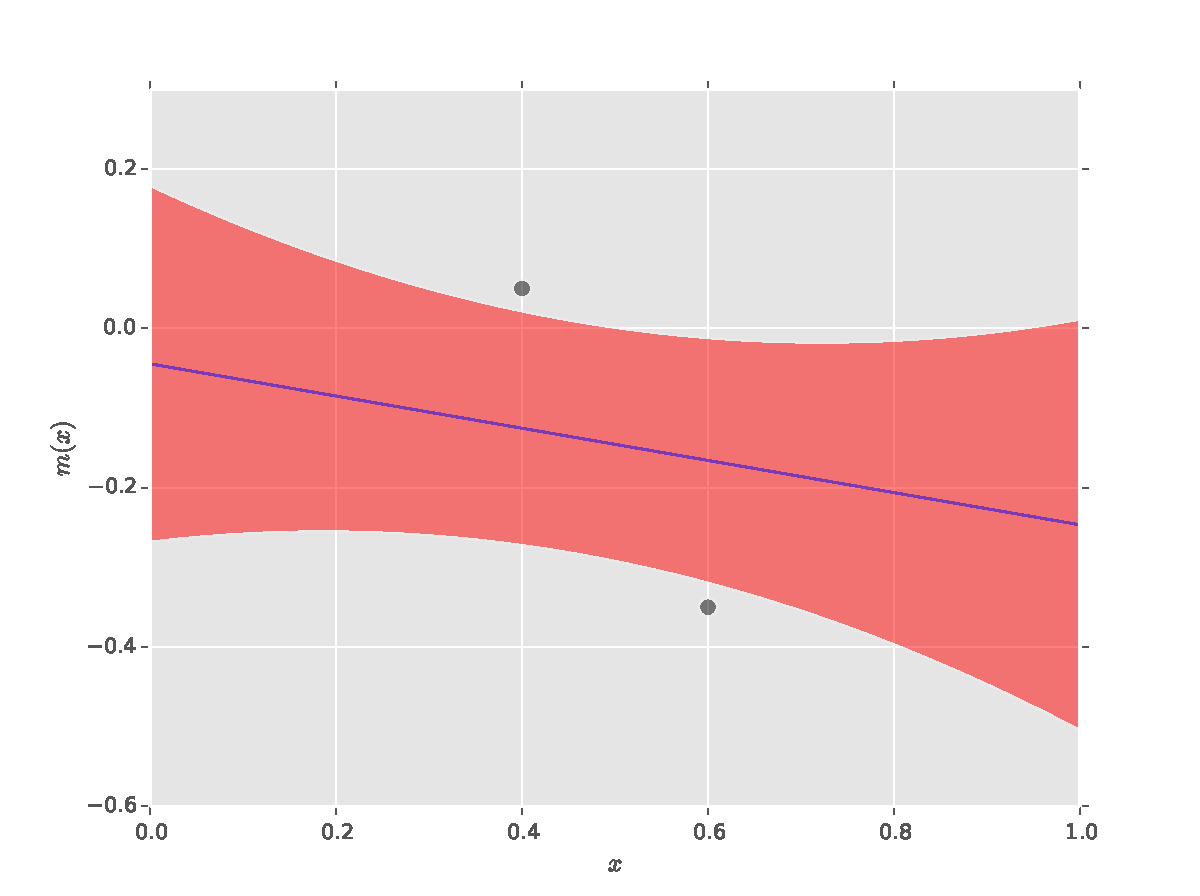
\includegraphics[scale=0.65]{exercise_12.pdf}
			\caption{The blue line indicates the mean of the predictive distribution plotted against x. The two gray dots are the data points and the red area indicates the standard deviation. The area is bound by the mean plus the standard deviation and by the mean minus the standard deviation.}
			\label{meanvar}
		  \end{figure}
	\item In figure \ref{sampled} some sampled linear equations are shown in green. The code snippet is shown below.

	\begin{verbatim}
		rands = np.random.multivariate_normal((-0.0445, -0.2021), inv(((22, 10), (10, 7.2))), 5)
	
		for r in rands:
		    x_range = np.linspace(0, 1, 100)
		    m_vals = np.array([np.dot(r.T, phi(x)) for x in x_range])
		    plt.plot(x_range, m_vals, alpha = 0.5, color='green')
	\end{verbatim}

	\begin{figure}[H]
			\centering
			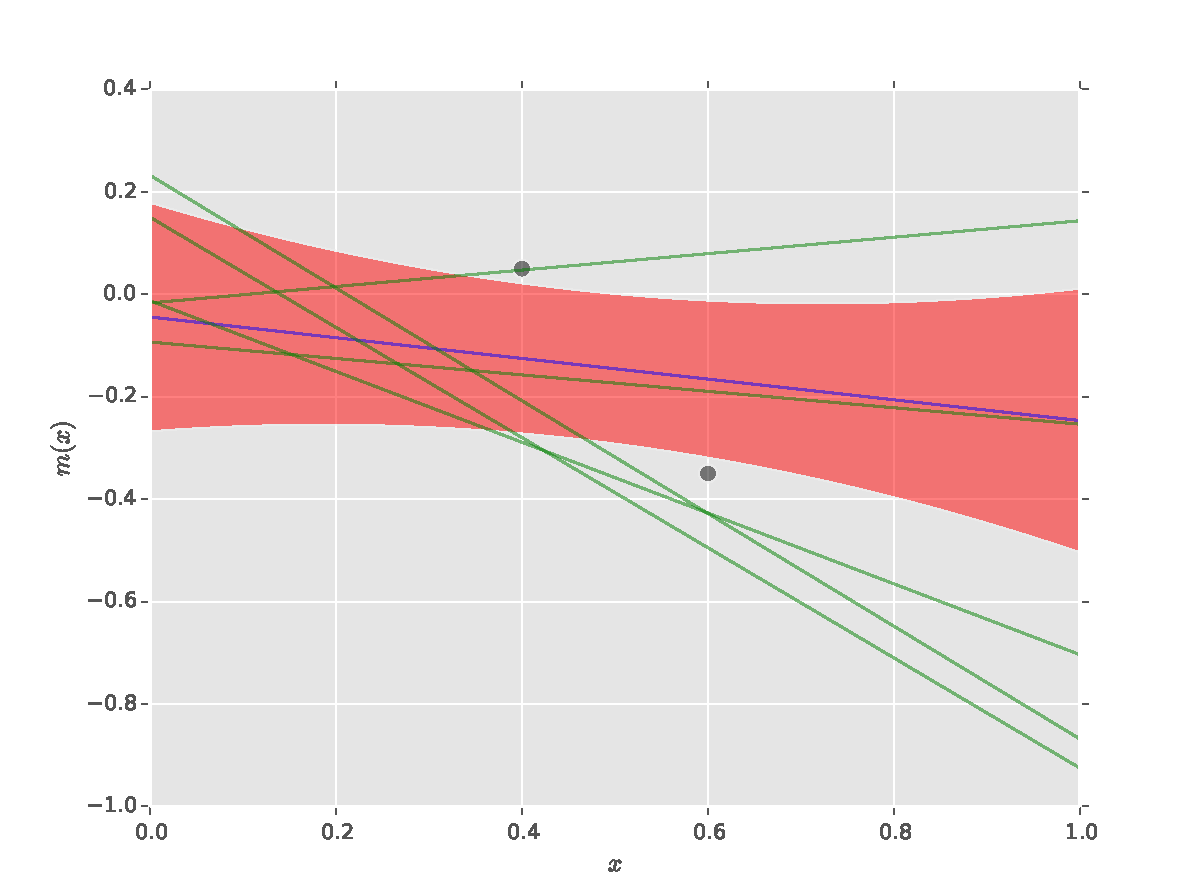
\includegraphics[scale=0.65]{exercise_13.pdf}
			\caption{The green lines represent $y(x, \boldsymbol w)$ where the weights $\boldsymbol w$ are sampled from the posterior distribution.}
			\label{sampled}
		  \end{figure}
\end{enumerate}

\section{Logistic regression}
\subsection{The IRLS algorithm}
\begin{enumerate}
	\item 
		We derive $f(x) = \sin(x)$, which gives $f'(x) = \cos(x)$, deriving this gives $f''(x) = -\sin(x)$.
		\begin{align}
			x^{(n+1)} &= x^{(n)} - \frac{f'(x^{(n)})}{f''(x^{(n)})}\\
			&= x^{(n)} + \frac{\cos(x^{(n)})}{\sin(x^{(n)})}
		\end{align}

		With the following Python code we can run several iterations easily:

		\begin{verbatim}
		from math import cos, sin

		def next(x):
		    return x + cos(x)/sin(x)

		if __name__ == "__main__":
		    x = 1
		    print x
		    for i in range(0, 5):
		        x = next(x)
		        print x
		\end{verbatim}

		The output for $x^{(0)} = 1$ is as follows:

		\begin{verbatim}
		1
		1.64209261593
		1.57067527716
		1.5707963268
		1.57079632679
		1.57079632679
		\end{verbatim}

		It looks like the value of $x$ converges after 4 iterations in this case. $\sin(x)$ has indeed $\approx 1.57$ as its maximum.

		For $x^{(0)} = -1$:

		\begin{verbatim}
		-1
		-1.64209261593
		-1.57067527716
		-1.5707963268
		-1.57079632679
		-1.57079632679
		\end{verbatim}

		In this case, the algorithm also converges after 4 iterations. Now, the value is a minimum of $\sin(x)$. This can be expected since this method does not differentiate between minimums and maximums. It finds the values where the derivative is 0, which is the case in both the maxima and minima of a function.
	\item
		Using the following Python code the value for $\boldsymbol w$ converges after approximately 6 iterations to $\approx [9.8, -21.7]$.
		\begin{verbatim}
def gradient(phi, y, t):
    return np.dot(phi.T, y - t)

def hessian(phi, y):
    R = np.diag(np.squeeze(y * (1-y))) # squeezing out extra dim. required for np.diag to work
    return np.dot(phi.T, np.dot(R, phi))

def sigmoid(x):
    return 1.0 / (1 + np.exp(-x))

if __name__ == "__main__":
    w = np.array([[1], [1]])
    x = np.array([0.3, 0.44, 0.46, 0.6])
    t = np.array([[1], [0], [1], [0]])
    phi = np.array([[1, xx] for xx in x])

    for i in range(0, 10):
        y = sigmoid(np.dot(phi, w))

        cur_gradient = gradient(phi, y, t)
        cur_hessian = hessian(phi, y)

        w = w - np.dot(inv(cur_hessian), cur_gradient)

        print w
		\end{verbatim}

		To show that $\phi = 0.45$ is the decision boundary, we need to check whether the probability of a data point with $\phi = 0.45$ is the same for $C_1$ and $C_2$. This consequently means that they should both be $0.5$ since $p(C_1 \vert \phi) + p(C_2 \vert \phi) = 1$.

		\begin{equation}
			p(C_1 \vert \phi) = y(\phi) = \sigma (\boldsymbol w^T \phi) = \sigma (\begin{pmatrix} 9.78227684 \\ -21.73839298 \end{pmatrix}^T \begin{pmatrix} 1\\0.45 \end{pmatrix}) = 0.50
		\end{equation}
\end{enumerate}

\subsection{Two-class classification using logistic regression}
\begin{enumerate}
	\item See figure \ref{scatter_iris}.

			\begin{figure}[H]
				\centering
				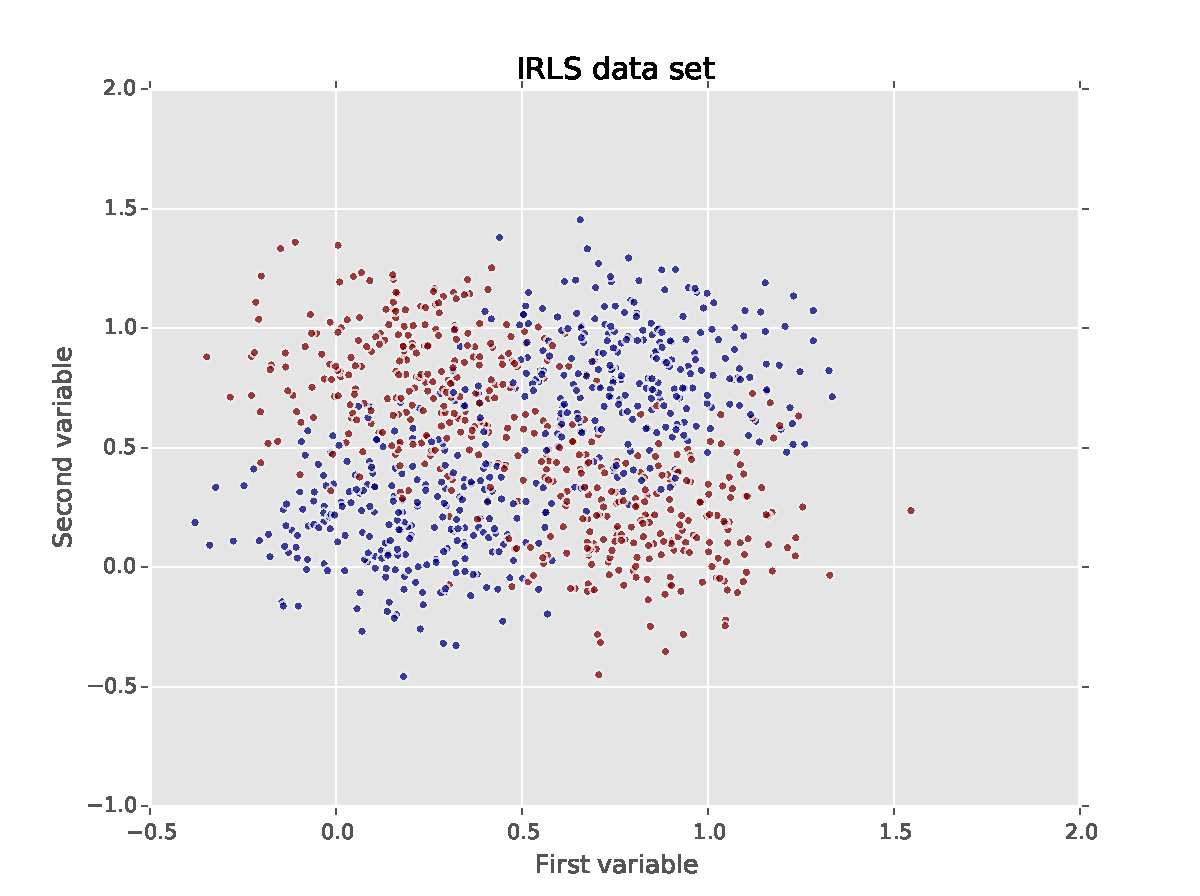
\includegraphics[scale=0.75]{exercise_221.pdf}
				\caption{Scatter plot of the IRLS data set.}
				\label{scatter_iris}
			\end{figure}
			I believe logistic regression can be a good fit for this problem since there is a clear pattern in the scatter plot. Some sort of Gaussian basis function could work well with the obvious densities as visible in the plot. A dummy basis function will not work since the problem is not seperable by a line.
	\item
		The class probabilities are all 0.5 since:
		\begin{equation}
			p(C_1 \vert \phi) = y(\phi) = \sigma (\boldsymbol w^T \phi) = \sigma (\begin{pmatrix} 0 \\ 0 \\ 0 \end{pmatrix}^T \phi) = \sigma (0) = 0.5
		\end{equation}
		The modifications that were needed to make the algorithm work are as follows:
		\begin{verbatim}
			w = np.array([[0], [0], [0]])     instead of
			    w = np.array([[1], [1]])

			phi = np.array([[1, xx[0], xx[1]] for xx in x])    instead of    
			    phi = np.array([[1, xx] for xx in x])
		\end{verbatim}
		The rest of the algorithm was already implemented in a way that handles multi-dimensional input data.
	\item
		The scatter plot can be found in figure \ref{scatter_dummy}. Darker colors indicate a higher probability for $C_1$. Note that the probabilities have been scaled to the range $0 < p(C_1 \vert \phi) < 1$ to show the differences between probabilities in the scatter plot. If we do not scale the values, there is no visible difference. In reality the probabilities range from $0.48$ to $0.51$. The scatter plot shows that logistic regression with this basic basis function does not perform well, as is to be expected.

		The obtained weights after 1000 iterations were:
		\begin{equation}
			\boldsymbol {\hat w} = \begin{pmatrix}
						0.00440664\\
						-0.02139153\\
						-0.04930069
					 \end{pmatrix}
		\end{equation}

		The cross entropy error for the initial weights was approximately $693.2$. The error after optimization was $692.9$.
		This proves the conclusions we drew from the scatter plot: logistic regression does not work well on this data set with this basic basis function.

		\begin{figure}[H]
			\centering
			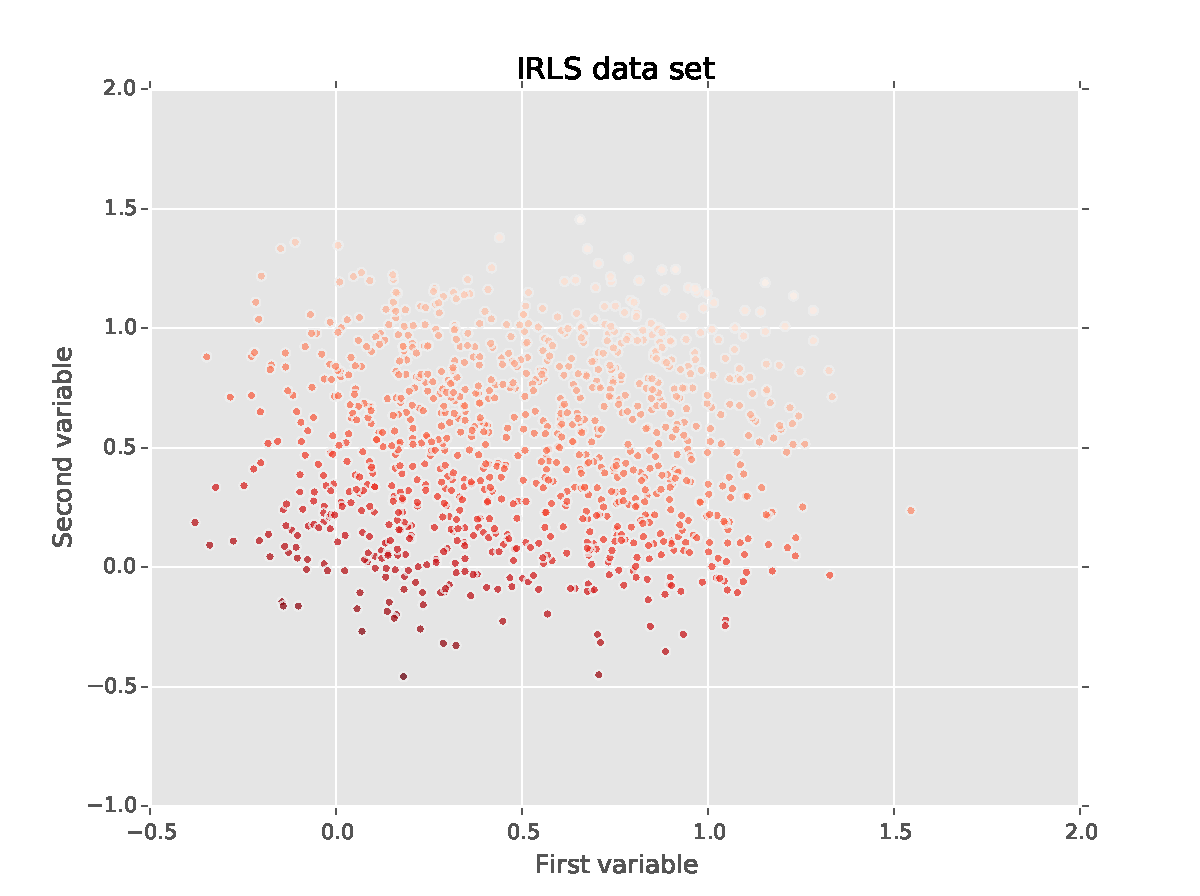
\includegraphics[scale=0.75]{exercise_223.pdf}
			\caption{Scatter plot of the IRLS data set. A darker color indicates a higher probability for $C_1$. Note that the probabilities are scaled, in reality they lie in the range $0.48 < p(C_1 \vert \phi) < 0.51$.}
			\label{scatter_dummy}
		\end{figure}
	\item
		Changing the previous basis function to the Gaussian basis function was very easy. The relevant lines of code are shown below. Note that the normalization of the Gaussian is not really necessary.

		\begin{verbatim}
			def gbf(x, m, s):
			    sigma = s * np.identity(np.array(m).shape[0])
			    a = (x-m)[np.newaxis].T
			    normalizer = 1.0 / (2*np.pi)**(a.shape[0]/2) * 1.0 / np.linalg.det(sigma)**(1/2)
			    return normalizer * np.exp(-(1.0/2)*np.dot(a.T, np.dot(inv(sigma), a)))

			phi = np.array([[1, gbf(xx, (0, 0), 0.2), gbf(xx, (1, 1), 0.2)] for xx in x])
		\end{verbatim}

		The scatter plot of the new feature space is shown below in figure \ref{scatter_gaussian}.

		\begin{figure}[H]
			\centering
			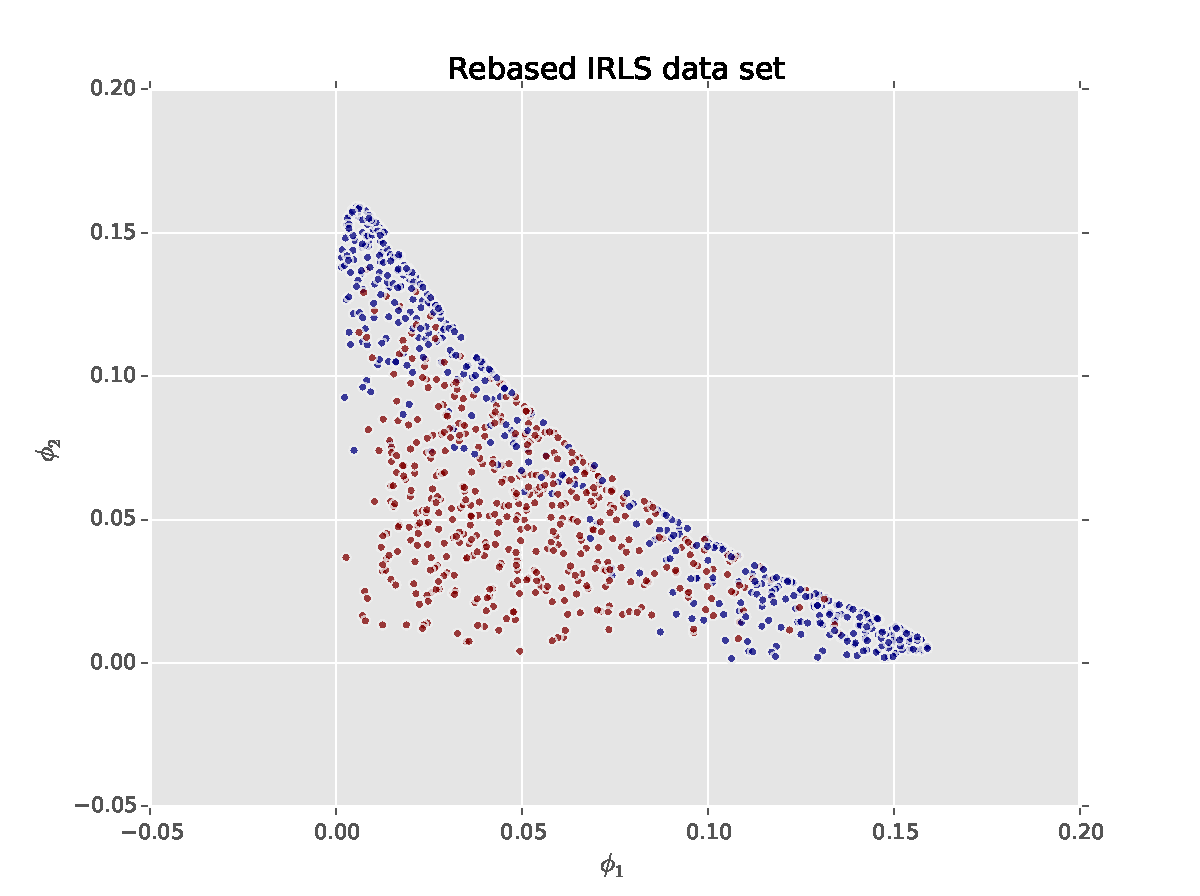
\includegraphics[scale=0.6]{exercise_224.pdf}
			\caption{The IRLS data set in the new feature space, based on $\phi_1$ and $\phi_2$. The color indicates whether a point has class $C_1$ or $C_2$.}
			\label{scatter_gaussian}
		\end{figure}
	\item
		I did not have to change my algorithm to use the Gaussian basis functions. It worked out of the box after the changes made in the previous exercise. The scatter plot can be found in figure \ref{scatter_gaussian_p}. The figure shows the probability of a data point having class $C_1$. A dark red color indicates a probability of 1 while a white color indicates a probability of 0 (and thus a high probability for $C_2$). A cross entropy error of $346.5$ was achieved, a significant improvement from the dummy basis function.

		The weights that were obtained:
		\begin{equation}
			\boldsymbol {\hat w} = \begin{pmatrix}
										7.10834887\\
						 				-77.10716735\\
						 				-77.69154604
 								   \end{pmatrix}
 		\end{equation}

 		This result is achieved after a mere 5 iterations. I also tried other iteration counts; $< 5$ iterations gave a higher cross entropy error, while $>= 5$ iterations all had approximately the same error. I tested between $1$ (milliseconds) and $10000$ (20 seconds) iterations.

		\begin{figure}[H]
			\centering
			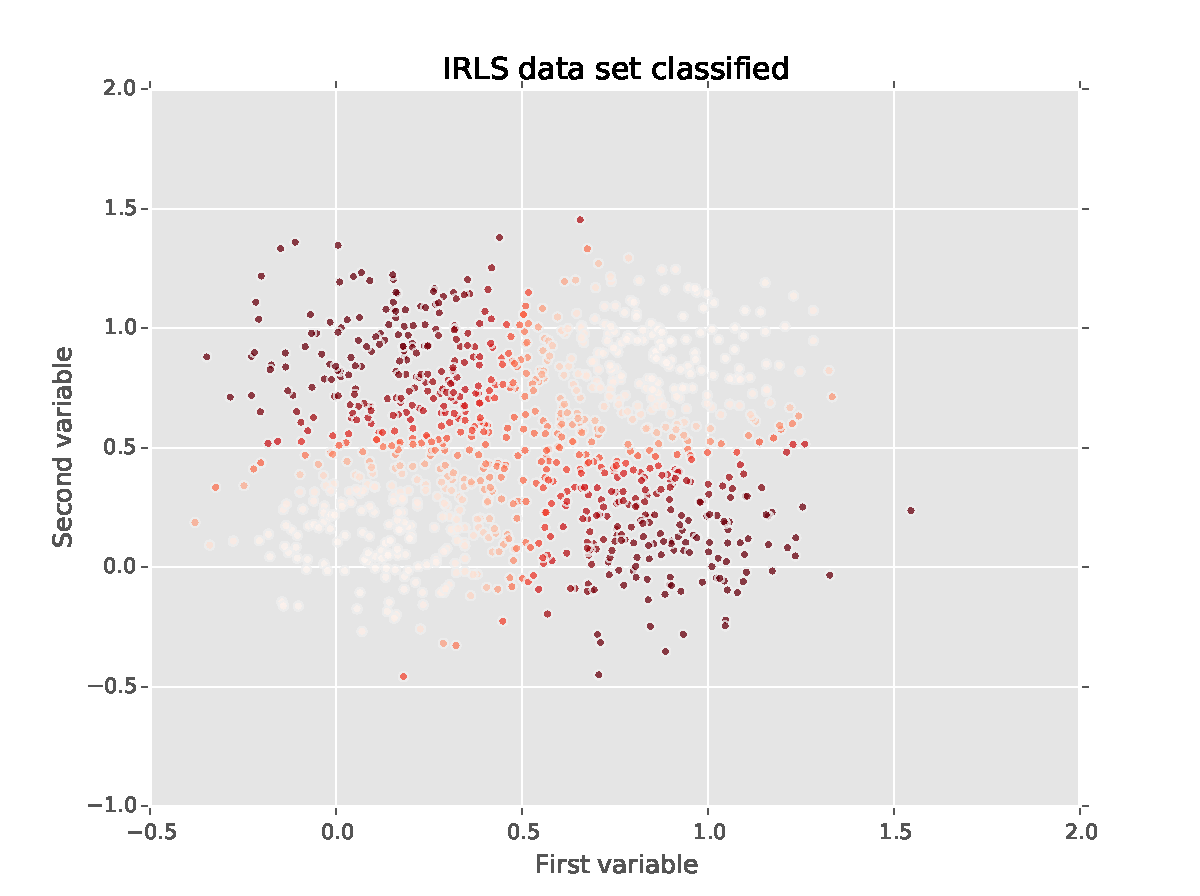
\includegraphics[scale=0.75]{exercise_225.pdf}
			\caption{The probabilities for each data point in the IRLS data set as classified by logistic regression using two Gaussian basis functions. A dark red color indicates a high probability for $C_1$ while a white color indicates a high probability for $C_2$. Probabilities are again scaled, although the effect of the scaling is a lot less than in the previous plot; the unscaled probabilities range from $0.0324$ to $0.999$.}
			\label{scatter_gaussian_p}
		\end{figure}
\end{enumerate}

\end{document}